\section{Motivation}

Buildings are notoriously complex from a management perspective.  They consume a large fraction
of the energy produced in the United States and much of is wasted~\cite{epa}.  There has been
much work in the building science community to reduce their energy consumption and make them more
efficieny, but the route to broader impact is typically carried out through regulations guided
by the findings of studies in those communities~\cite{regulation}.
We aim to let solutions reach buildings \emph{directly} by making sense of the data they produce
as quickly and accurately as possible.
In order to achieve this at scale, we must explore ways to deal with the data produced
from sensors within them and to enable braod anaysis across several buildings at a time. Our study
focuses on any building equipped with a network of sensors.  Nearly 
three-quarters of commercial buildings contain a rich sensing fabric, installed as part
of the building management system~\cite{study}.  
It is the data from these system and variants of it, that
we wish to unify and make sense of in a more systematic and automated fashion.

Fortunately, we have access to a large corpus of data from buildings on our campus.
We examine the data from 56 buildings containing over 22,600 sense points. These buildings 
represent a vast range in age, size, and density of deployment.  It also represents deployments
that were set up by more than one vendor.  As expected, newer buildings have many more sense 
points than older ones -- although some old buildings that have been retrofitted have over 1000  
points within them. The maximum number of points in a 
single building is 6169 and the minimum is 27.   The built years spans over 100 years -- from 
1905 to 2007. The size range spans over an order of magnitude 
in square footage from about 30,000 square feet to over 360,000 square feet.  The access this
this kind of breadth of system and building types makes our study unique.

\begin{figure*}[h]
\centering
	\begin{subfigure}{0.5\textwidth}
                \centering
		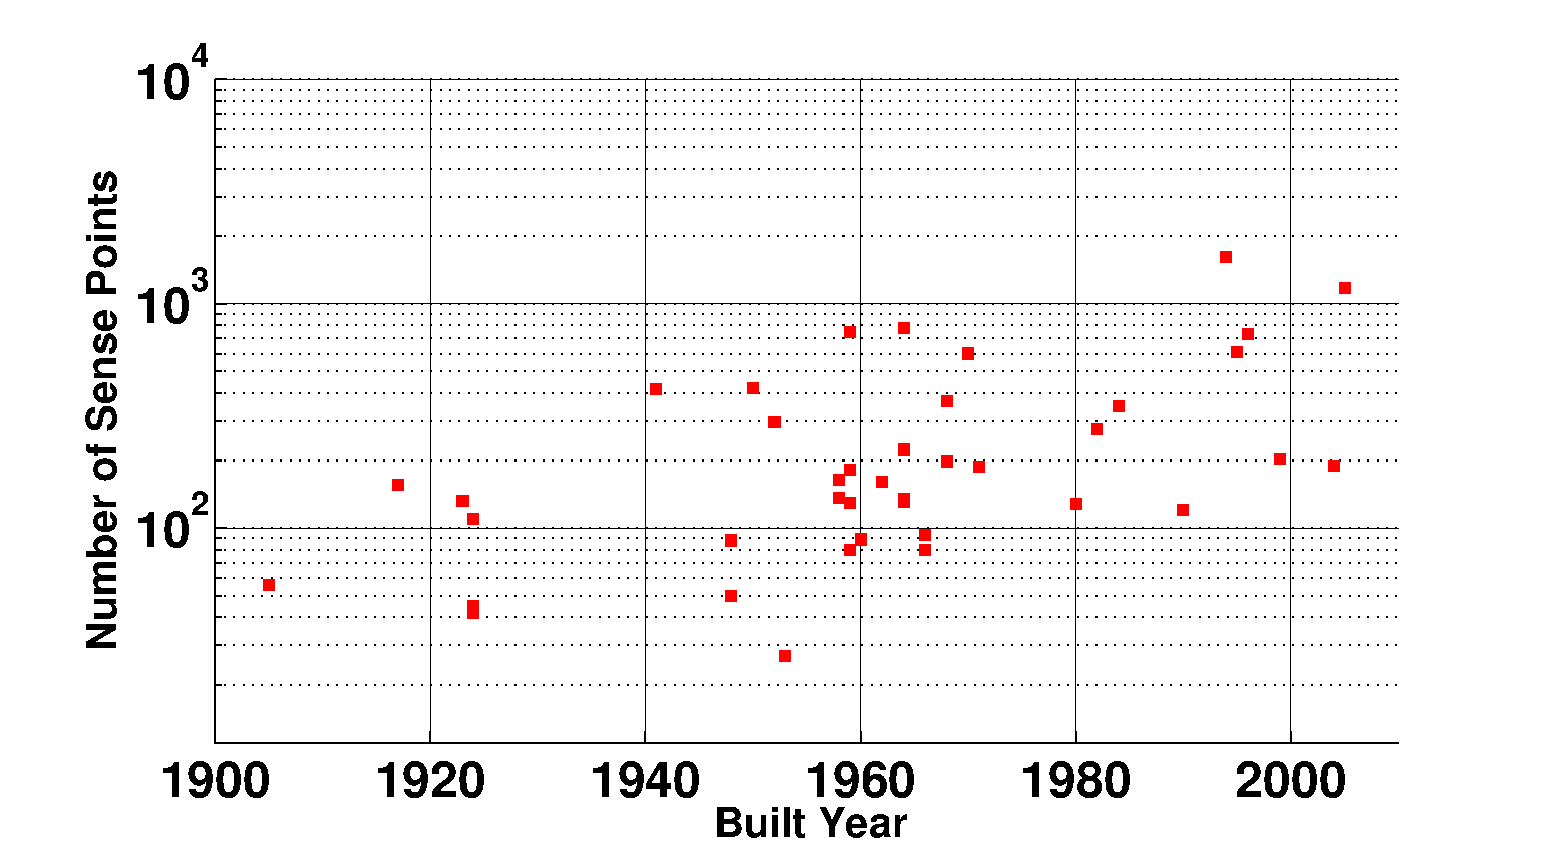
\includegraphics[width=\textwidth]{./figs/pts_vs_yearbuilt.eps}
                \caption{Number of Points vs Year Built}
	\end{subfigure}
	\begin{subfigure}{0.5\textwidth}
                \centering
		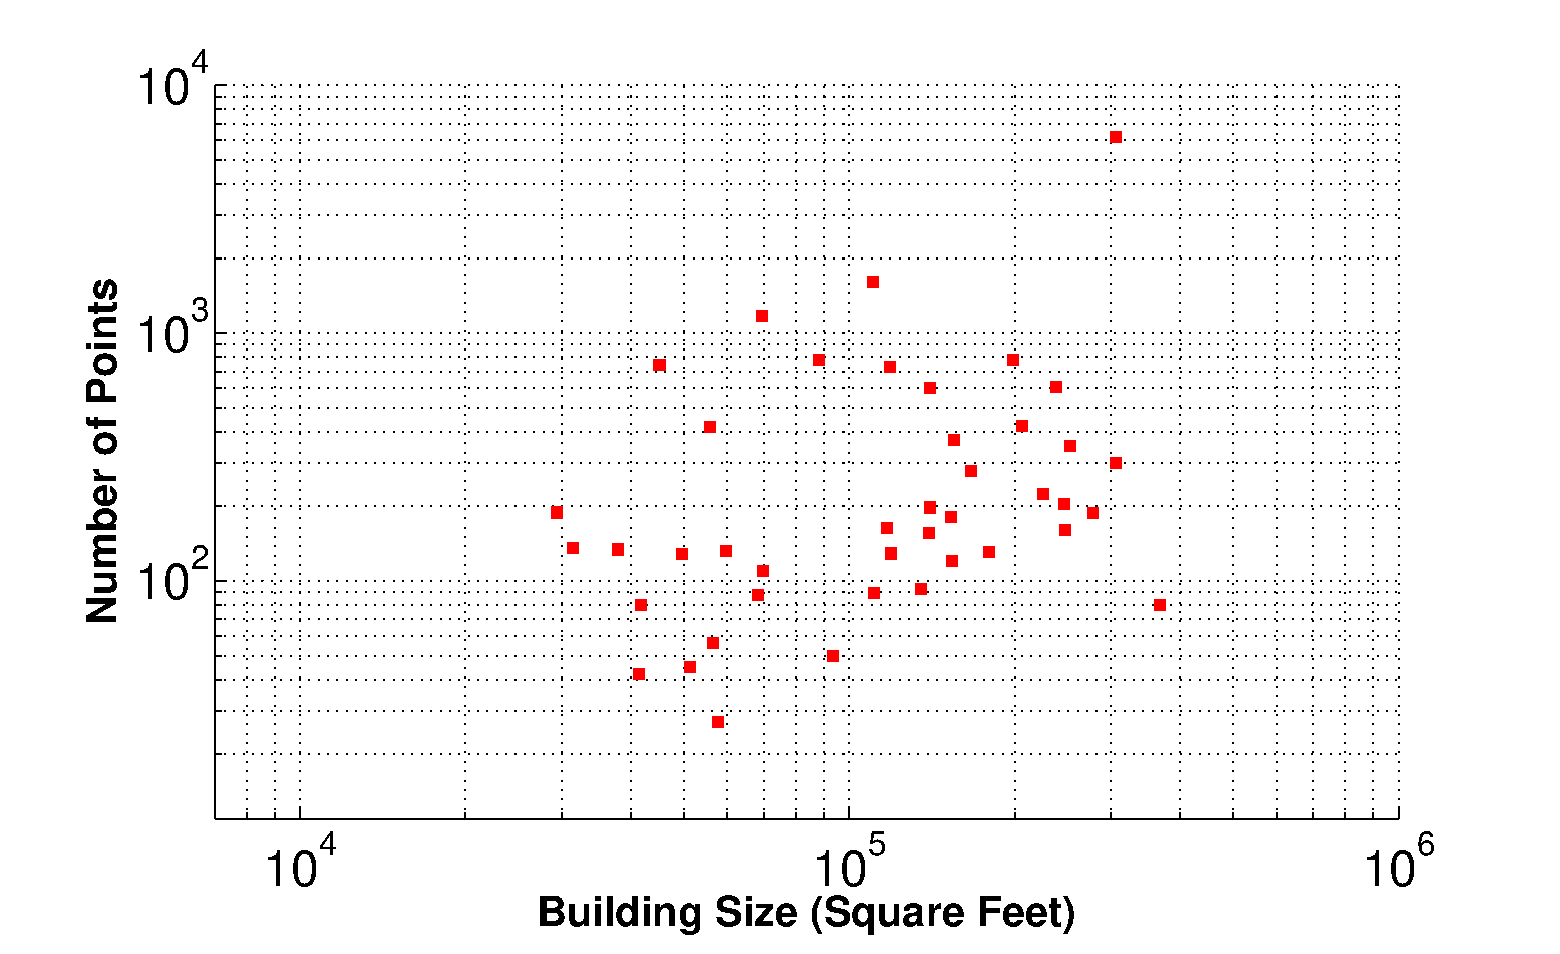
\includegraphics[width=\textwidth]{./figs/pts_vs_buildsz.eps}
                \caption{Number of Points vs Building Size}
	\end{subfigure}
\caption{}
\label{fig:sense_pts_data}
\end{figure*}



% walk through an example of point names from 2 or three buildings and explain 
% what's challenging here
%
% BLDA1R435__ART
% BLDA1R435__ARS
% BLDA1R545__ART
%Buildings consume a large fraction of the energy produced in the United States, and much of it
%is wasted\cite{epa}.  
As mentioned, buildings are notoriously complex and  ad-hoc data management practices
make it difficult for any analytical solution to be widely ported or run across building
systems.  For example, consider the following stream names: \texttt{BLDA1R435\_\_ART,
BLDA1R435\_\_ARS, BLDA1R545\_\_ART}. Each name encodes contextual information in the form
of concatinated character sequences. In these, the first 4 characters refer to the 
name of the building, the next one encodes the air handling unit association, the next 
four encode the room,
and the last three encode the acronym for the type.  Although the examples given are well
structured, many variants within the same data set exist.  For example, \texttt{BLD\_1R435\_ARG\_}
is the encoding for a different sensor in the same room as the others, but with a name
that is \emph{like} although not exactly the same structure as the others.

% Discuss how active learning technique can be used to "unify" these tag names

When dealing with a small number of points such differences are usually not a problem.  Upon 
visual inspection, the two
encodings are similar enough that the engineer can decode the meaning.  However, for automatic 
processing or processing a large number of points, these kinds of variations makes it difficult 
to generalize the character-contruction
rule set.  Without rule-set construction the data cannot be ingested properly or interpretted
correctly.  However, there are ``active learning'' techniques in the literature~\cite{ms} 
that address this problem by leveraging the knowledge of an expert. The idea behind active learning
is that you can request input from an expert to improve the accuracy of your algorithm.
In the case of name/tag expansion you 
can generalize the set of rules that generate a name/tag by example, iteratively
updating the name construction rule set for different types of names.  An expert feeds
the system examples of names for a particular type of sensor or code, and the algorithms 
that generalize the character-set construction rules can raise the confidence of the
expanded expression.
We explore the use
of \emph{active learning} techniques to iteratively learn all the variants within an across
data sets.

% expand the discussion to include sensor sin iot?


% Now discuss how the actual shapes of the readings can be quite similar looking

%\begin{figure}[h!]
%\centering
%    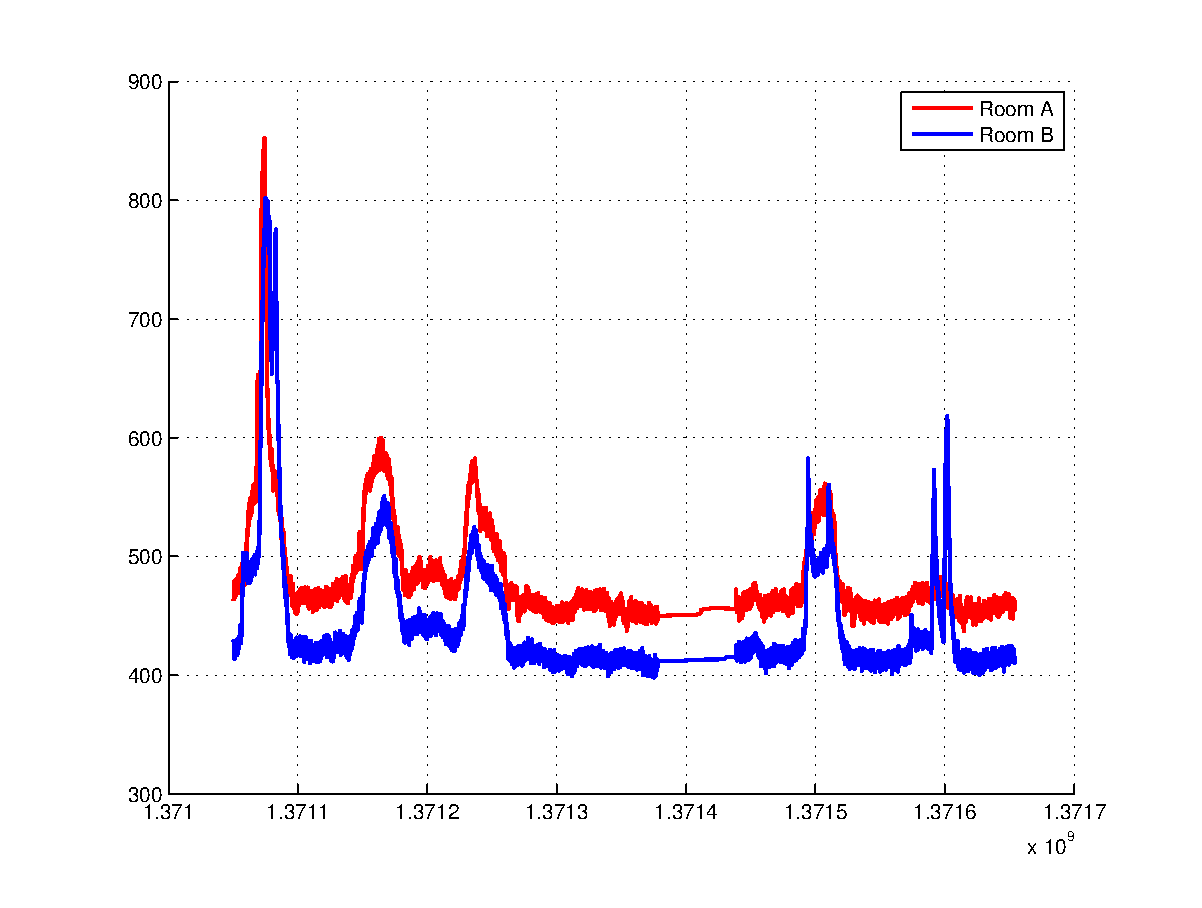
\includegraphics[width=0.48\textwidth]{figs/co2_pair.eps}
%    \caption{CO2 sensor traces.}
%\label{fig:co2traces}
%\end{figure}
%
%\begin{figure}[h!]
%\centering
%    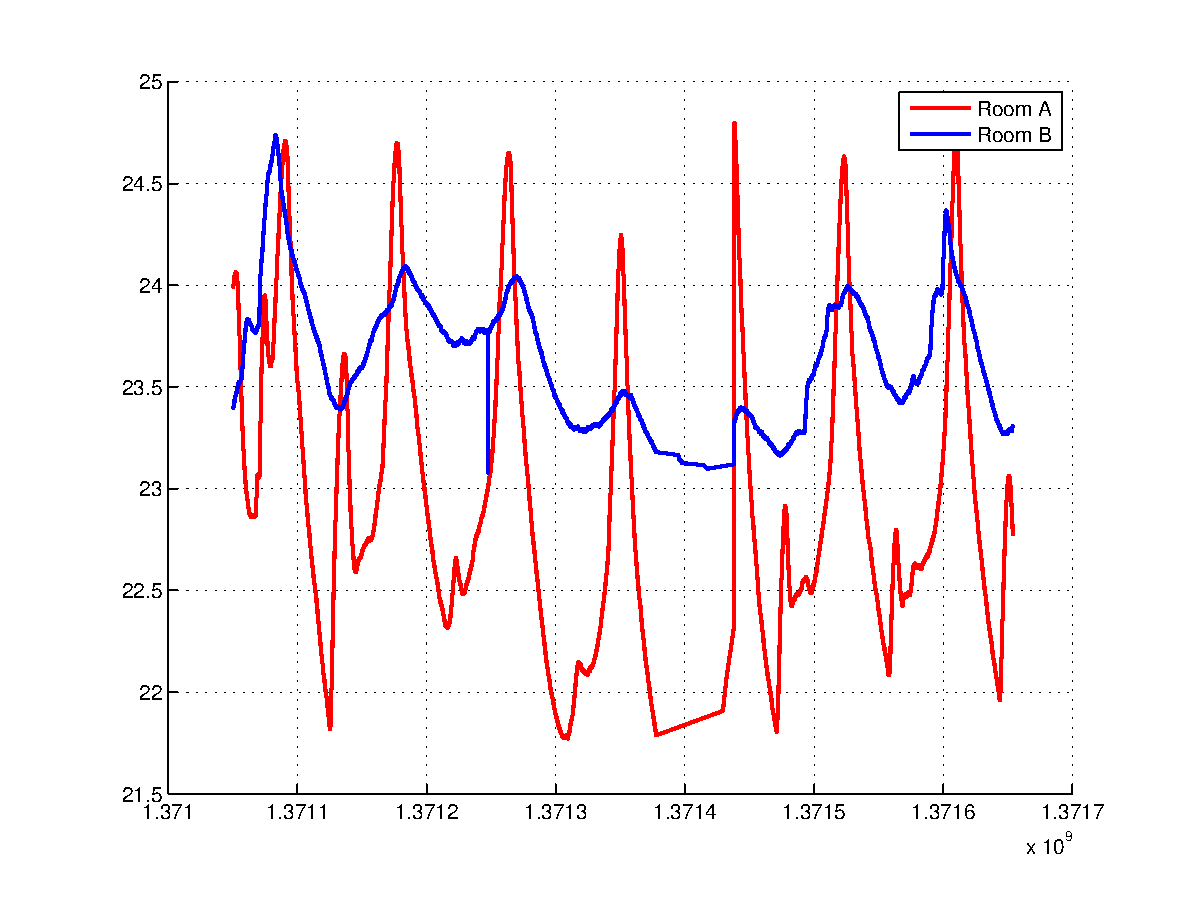
\includegraphics[width=0.48\textwidth]{figs/temp_pair.eps}
%    \caption{temperature traces.}
%\label{fig:temptraces}
%\end{figure}

% tie this into search; search is done for scale
% scale is necessary for broad impact
% 

% discuss how both can be used to generate more metadata that we can use for indexing


